%overall
\begin{frame}[c,fragile]{Validation of the technique: gripper-door}
\begin{columns}[T]
    \begin{column}<1->{0.5\textwidth}
        \centering

        \begin{overprint}
            \onslide<1>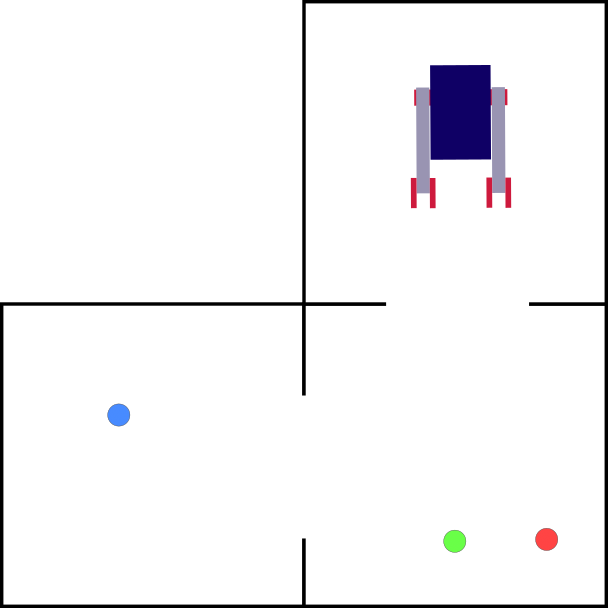
\includegraphics[width = 0.8\textwidth]{images/3_rooms/gd_3_0.png}
            \onslide<2>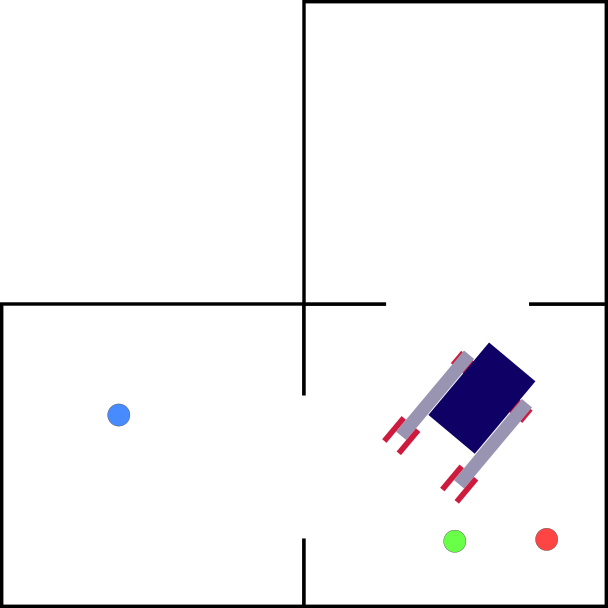
\includegraphics[width = 0.8\textwidth]{images/3_rooms/gd_3_1.png}
            \onslide<3>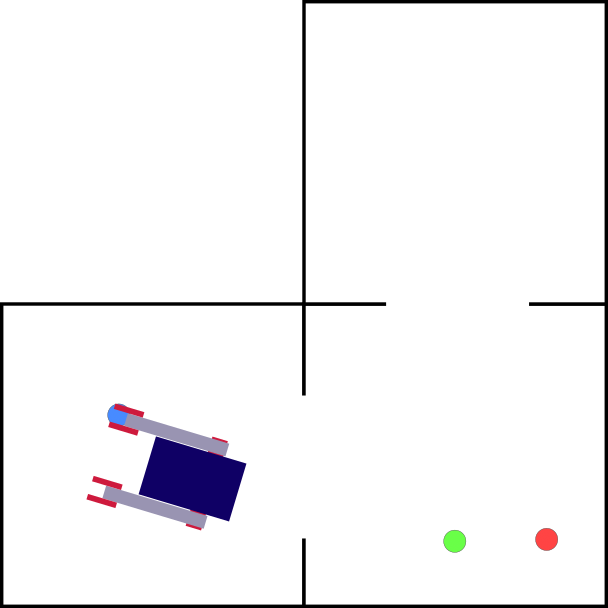
\includegraphics[width = 0.8\textwidth]{images/3_rooms/gd_3_3.png}
            \onslide<4->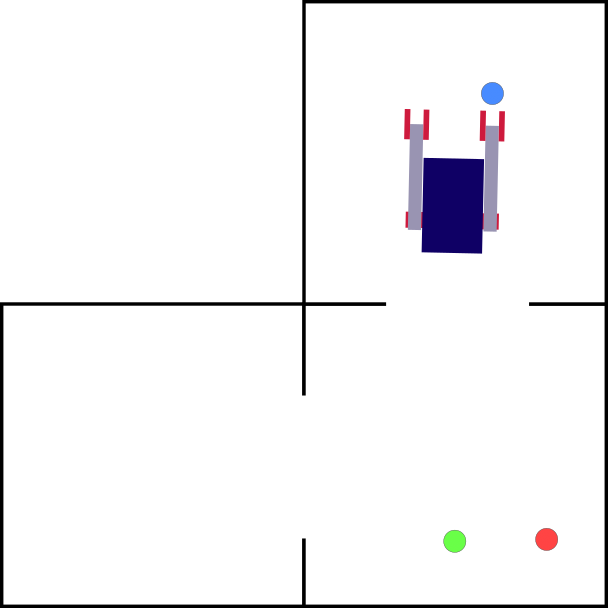
\includegraphics[width = 0.8\textwidth]{images/3_rooms/gd_3_6.png}
        \end{overprint}
    \end{column}
    \begin{column}<1->{0.5\textwidth}
        A \textit{robot} needs to place \textit{balls} in different \textit{rooms}
        \small
        \onslide<1->
        \begin{itemize}
            \item Actions:
            \onslide<2-> move
            \onslide<3->, pick
            \onslide<4-> , drop
            \onslide<5->
            \item State-functions:
                \begin{itemize}
                    \item at({ball, robot}) location
                    \item carry(?ball) gripper
                    \item connected
                \end{itemize}
            \item Tasks and methods: pick-and-drop(m1, m2), t\_move(m\_recursive, m\_already\_there)   
        \end{itemize}
    \end{column}
    
\end{columns} 
\end{frame}

\begin{frame}[c, fragile]{Problems of different sizes}
    \begin{columns}[c]
        \begin{column}[c]{0.3\textwidth}
            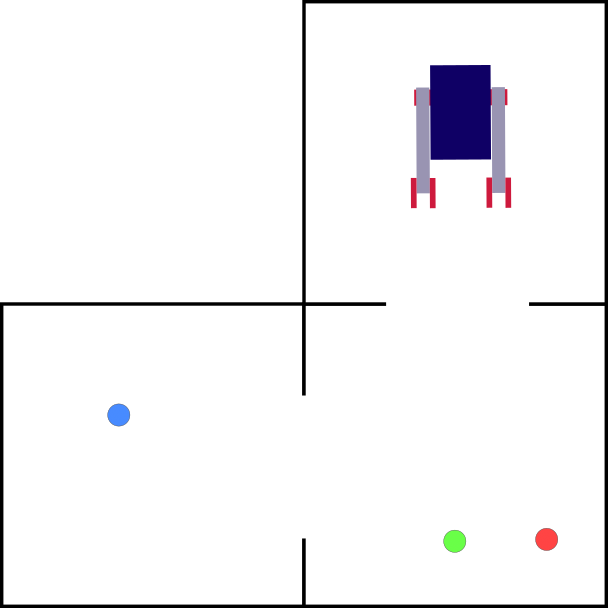
\includegraphics[width = 0.8\textwidth]{images/3_rooms/gd_3_0.png}
        \end{column}
        \begin{column}{0.1\textwidth}
            \centering $\rightarrow$
        \end{column}
        \begin{column}[c]{0.5\textwidth}
            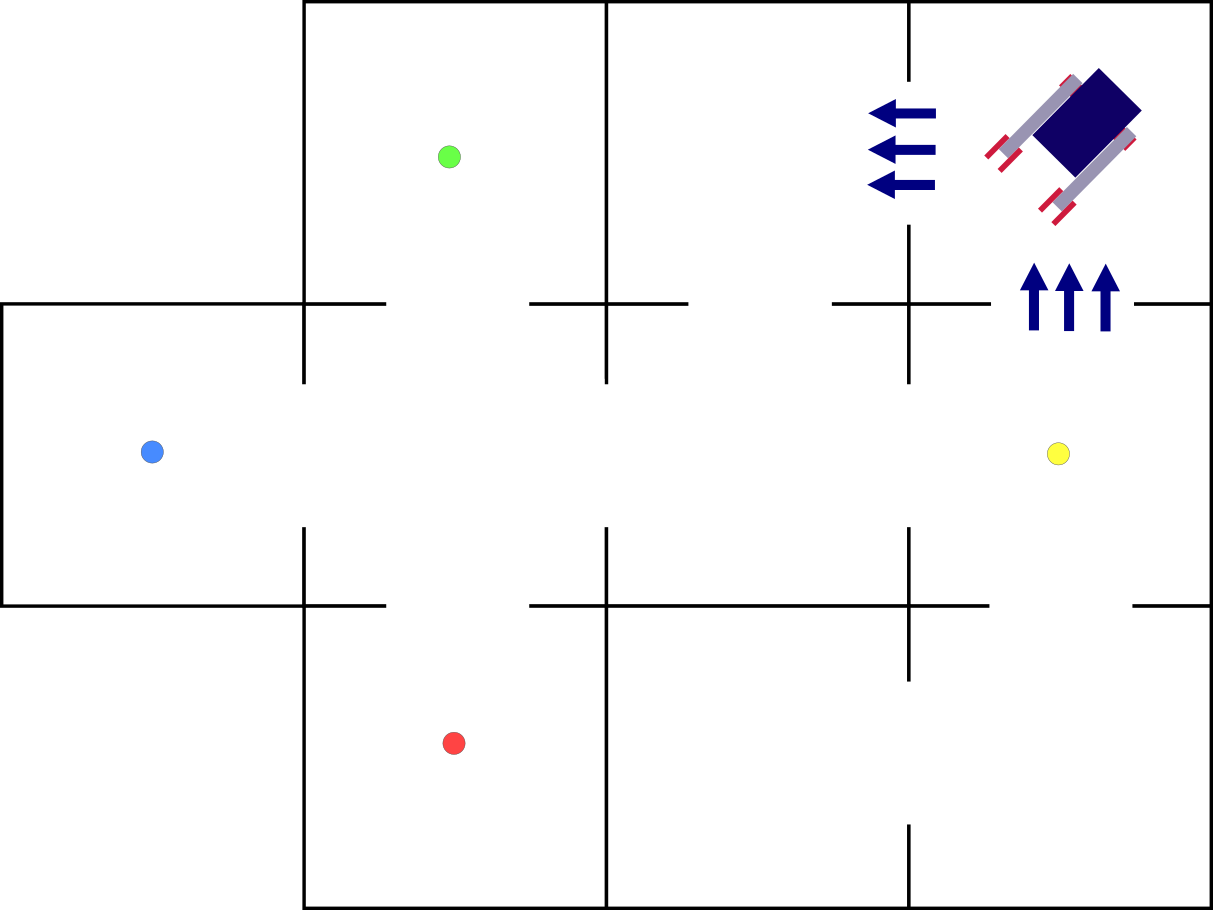
\includegraphics[width = \textwidth, angle=90]{images/11_rooms/gd_11_0.png}
        \end{column}
    \end{columns}
\end{frame}